\documentclass[aspectratio=169,fleqn]{beamer}
\PassOptionsToPackage{english}{babel}
\usepackage{standardslides}

\usepackage{svg}

\usepackage{tikz}
\usepackage{pifont}
\usepackage{listings}
\usepackage{colortbl}
\newlength{\listingframemargin}
\setlength{\listingframemargin}{1em}
\newlength{\listingmargin}
\setlength{\listingmargin}{0.08\textwidth}

\definecolor{codeDarkGray}{gray}{0.2}
\definecolor{codeGray}{gray}{0.4}
\definecolor{codeLightGray}{rgb}{0.94,0.94,0.91}
\definecolor{codeBorder}{rgb}{0.34,0.24,0.21}
\definecolor{MidnightBlue}{rgb}{0.1, 0.1, 0.8}

\lstdefinestyle{standard}{%
  belowcaptionskip=0.5\baselineskip,
  breaklines=true,
  frameround=tttt,
  % frame=false,
  xleftmargin=0em,
  xrightmargin=0em,
  showstringspaces=false,
  showtabs=false,
  % tab=\smash{\rule[-.2\baselineskip]{.4pt}{\baselineskip}\kern.5em},
  basicstyle= \fontfamily{pcr}\selectfont\tiny\bfseries,
  keywordstyle= \bfseries\color{MidnightBlue}, %\color{codeDarkGray},
  commentstyle= \itshape\color{codeGray},
  identifierstyle=\color{codeDarkGray},
  stringstyle=\color{BurntOrange}, %\color{codeDarkGray},
  numberstyle=\tiny\ttfamily,
  % numbers=left,
  numbersep = 1em,
  % stepnumber = 1,
  % captionpos=t,
  tabsize=2,
  % backgroundcolor=\color{codebLightGray},
  rulecolor=\color{codeBorder},
  framexleftmargin=\listingframemargin,
  framexrightmargin=\listingframemargin
}

\newcommand{\inputCodeBlock}[1]{%
  % \begin{mybox}
    \begin{center}
      % \begin{minipage}[c]{0.7\textwidth}
        \lstinputlisting[%
          style = standard,
          language = c++,
          morekeywords={constexpr,noexcept,decltype,size_t,uint32_t,uint64_t,__m256i,__m256,__m256d,__m128i,__m128,__m128d}
        ]{#1}
      % \end{minipage}
    \end{center}
  % \end{mybox}
}

% \def\UrlBigBreaks{\do\/\do-\do:}
\usepackage{xurl}

\setbeamertemplate{background}{
  
\includegraphics[width=\paperwidth,height=\paperheight]{images/background-tessellation.png}
}

\setbeamertemplate{footline}[frame number]
\setbeamertemplate{navigation symbols}{}

\title{%
  Workshop Version Control: \\ Getting Started with Git%
}
% \subtitle{Master's Thesis Defense and Presentation}
\author{Markus Pawellek}

\bibliography{references}

\begin{document}

\selectlanguage{english}

\begin{frame}[plain]
  
\includegraphics[width=0.2\linewidth]{images/logo.png}
  \hfill
  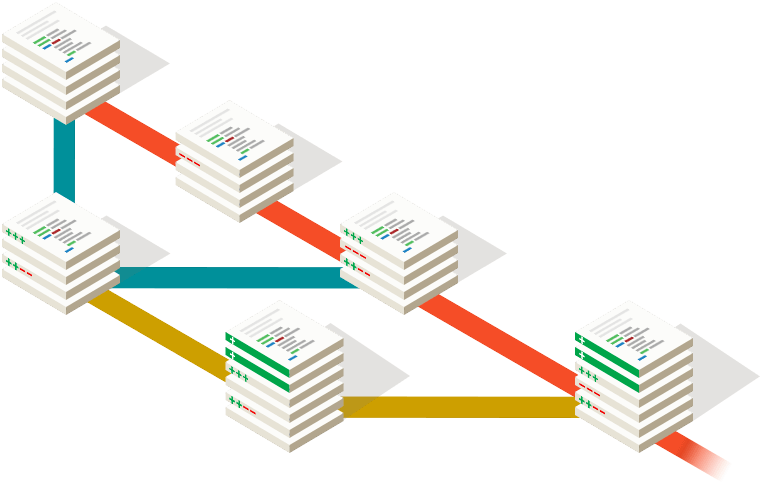
\includegraphics[width=0.7\linewidth]{images/banner.png}
\end{frame}

\frame[plain]{\titlepage}

\begin{frame}[plain]{Outline}
  \footnotesize
  \hfill\parbox[t][7cm][l]{0.9\textwidth}{\tableofcontents}
\end{frame}

\setcounter{framenumber}{0}

\section{Motivation} % (fold)
\label{sec:motivation}

  \begin{frame}[plain]{}
    \centering
    
\includegraphics[height=0.85\textheight]{images/bad-version-control-1.jpg}

    {\scriptsize Image from \fullcite{bad-version-control}.}
  \end{frame}

% section motivation (end)

\section{Literature and Resources} % (fold)
\label{sec:literature_and_resources}

  \begin{frame}{Literature and Resources}
    \begin{itemize}
      \item \fullcite{git-homepage}
      \item \fullcite{git-reference}
      \item \fullcite{pro-git}
      \item \fullcite{github-docs}
      \item \fullcite{github-git-cheatsheet}
    \end{itemize}
  \end{frame}

% section literature_and_resources (end)

\section{Basics} % (fold)
\label{sec:basics}

  % \begin{frame}{Basics}
  %   
\includegraphics[width=0.2\linewidth]{images/logo.png}
  %   \hfill
  %   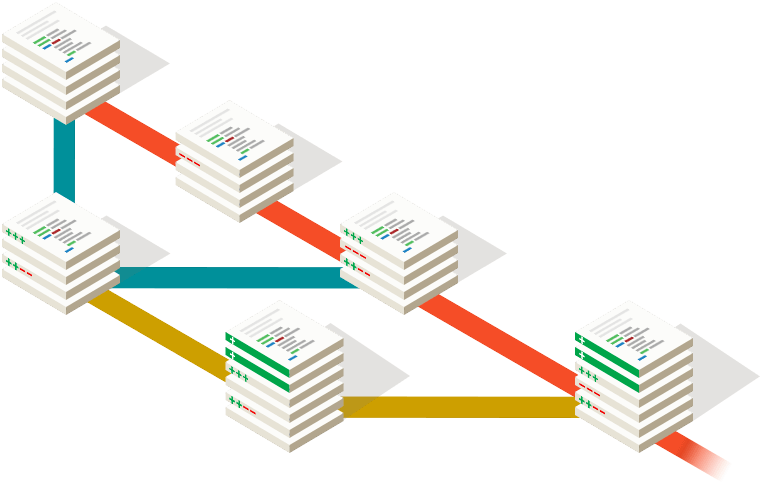
\includegraphics[width=0.7\linewidth]{images/banner.png}
  % \end{frame}

  \begin{frame}{Basics: Distributed Version Control}
    \centering
    \only<1>{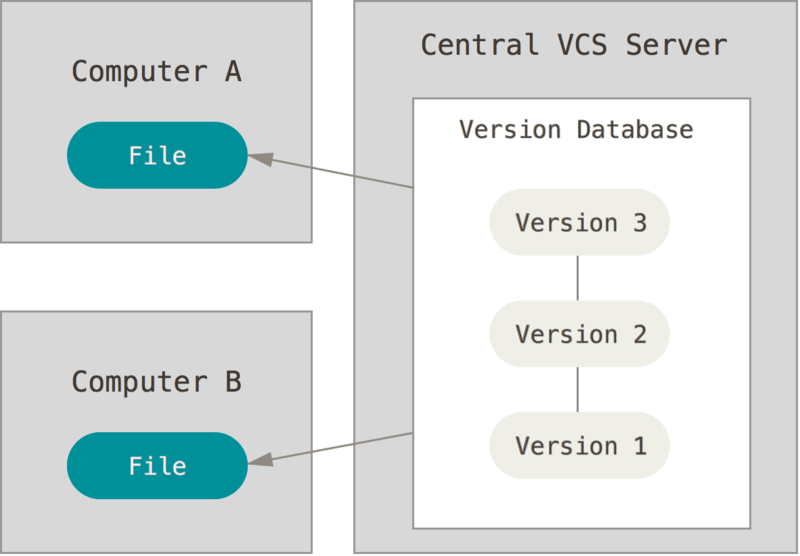
\includegraphics[height=0.8\textheight]{images/centralized.png}}
    \only<2>{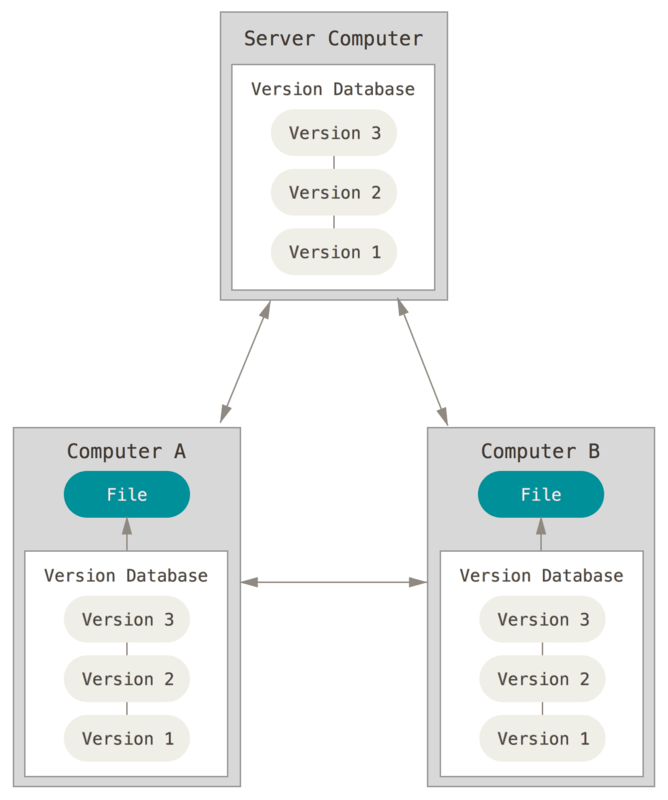
\includegraphics[height=0.8\textheight]{images/distributed.png}}

    {\scriptsize Image from \textcite{pro-git}.}
  \end{frame}

  \begin{frame}{Basics: Snapshots}
    \centering
    \only<1>{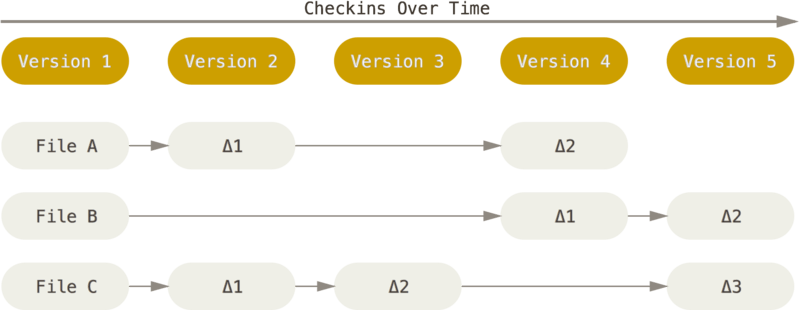
\includegraphics[width=0.8\linewidth]{images/deltas.png}}
    \only<2>{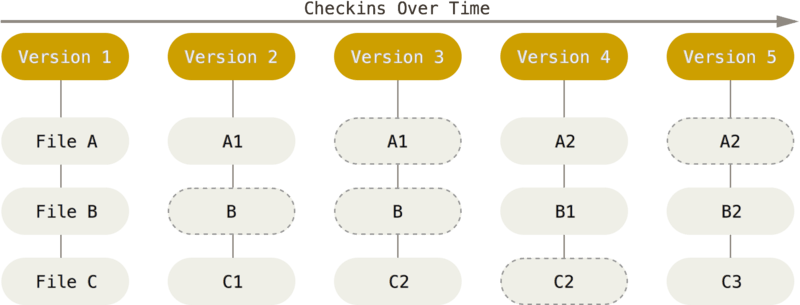
\includegraphics[width=0.8\linewidth]{images/snapshots.png}}

    {\scriptsize Image from \textcite{pro-git}.}
  \end{frame}

  \begin{frame}{Basics: The Three States}
    \centering
    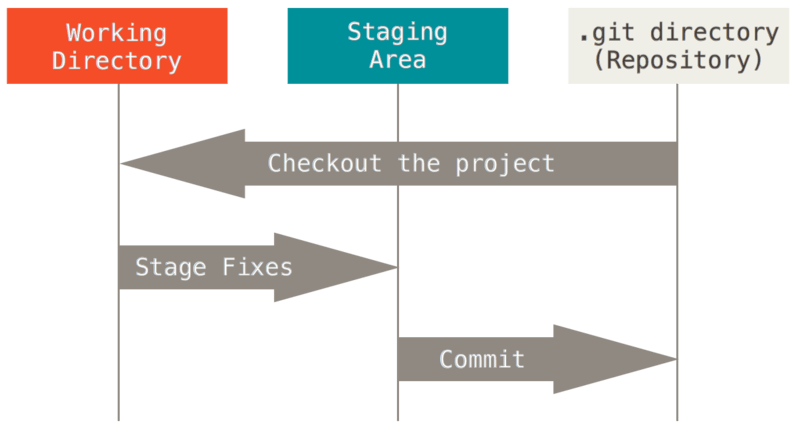
\includegraphics[height=0.8\textheight]{images/areas.png}

    {\scriptsize Image from \textcite{pro-git}.}
  \end{frame}

  \begin{frame}{Basics: Recording Changes}
    \centering
    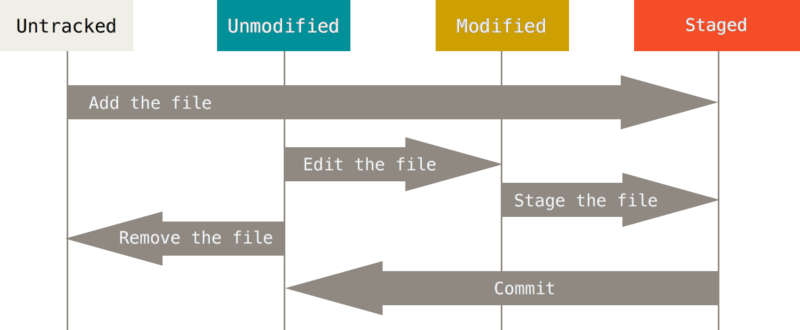
\includegraphics[width=\linewidth]{images/lifecycle.png}

    {\scriptsize Image from \textcite{pro-git}.}
  \end{frame}

  \begin{frame}{Basics: Commits}
    \centering
    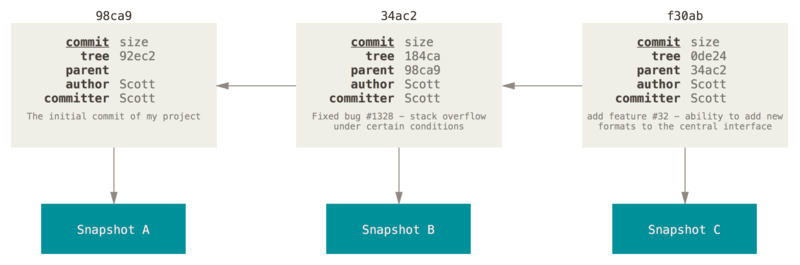
\includegraphics[width=\linewidth]{images/commits-and-parents.png}

    {\scriptsize Image from \textcite{pro-git}.}
  \end{frame}

  \begin{frame}{Basics: Commit Tree}
    \centering
    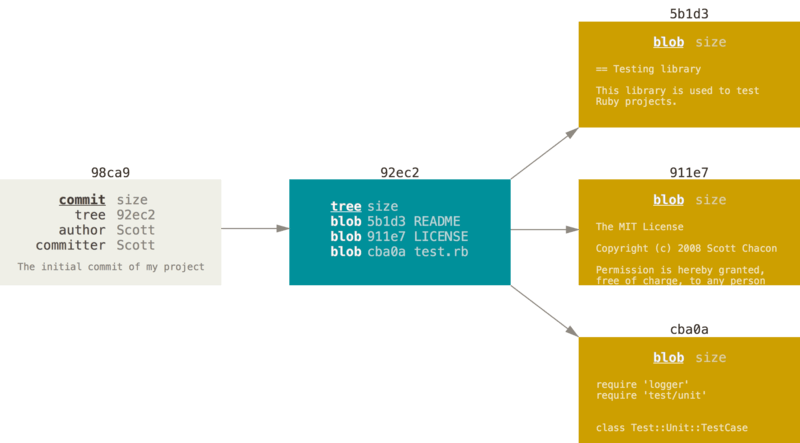
\includegraphics[height=0.8\textheight]{images/commit-and-tree.png}

    {\scriptsize Image from \textcite{pro-git}.}
  \end{frame}

% section basics (end)

\section{Git by Example} % (fold)
\label{sec:git_by_example}

  \begin{frame}{Git by Example}
    \begin{enumerate}
      \item Initial Setup
      \item Initializing Repositories
      % \item Commiting Files
      \item gitignore
    \end{enumerate}
  \end{frame}

% section git_by_example (end)

\section{Rules of Thumb} % (fold)
\label{sec:rules_of_thumb}

  \begin{frame}{Rules of Thumb: Commit Messages}
    \centering
    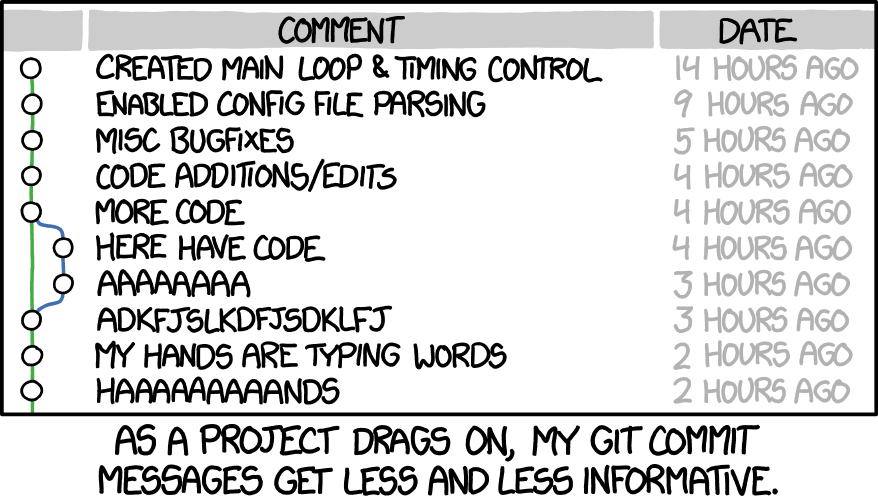
\includegraphics[height=0.8\textheight]{images/bad-commit-messages.png}

    {\scriptsize Image from \textcite{good-commit-message}.}
  \end{frame}

  \begin{frame}{Rules of Thumb: Commit Messages}
    The seven rules of a great Git commit message
    \begin{enumerate}
      \item Separate subject from body with a blank line
      \item Limit the subject line to 50 characters
      \item Capitalize the subject line
      \item Do not end the subject line with a period
      \item Use the imperative mood in the subject line
      \item Wrap the body at 72 characters
      \item Use the body to explain what and why vs. how
    \end{enumerate}
  \end{frame}

  \begin{frame}{Rules of Thumb}
    \begin{enumerate}
      \item Use gitignore whitelisting
    \end{enumerate}
  \end{frame}

% section rules_of_thumb (end)

\section{Outlook} % (fold)
\label{sec:outlook}

  \begin{frame}{Outlook}
    \begin{itemize}
      \item Submodules
      \item Hooks
      \item Merge and Rebase
      \item Cherrypick
      \item Stashing
      \item Signing your Work
      \item Searching
      \item Attributes
    \end{itemize}
  \end{frame}

% section outlook (end)

\setcounter{backupcounter}{\value{framenumber}}

\begin{frame}[plain]
  \vfill
  \centering
  \begin{beamercolorbox}[sep=8pt,center,shadow=true,rounded=true]{title}
    \usebeamerfont{title}%
    Thank you for Your Attention!%
    \par%
  \end{beamercolorbox}
  \vfill
\end{frame}

\begin{frame}[plain]
  \frametitle{References}
  % \tiny
  \AtNextBibliography{\tiny}
  \begin{multicols}{2}
    \nocite{*}
    \printbibliography
  \end{multicols}
\end{frame}

\setcounter{framenumber}{\value{backupcounter}}

\end{document}
